\chapter{Experimental Evaluation}
\label{chap:exp-eval}
The algorithms proposed in \autoref{chap:arch-syn} are experimentally evaluated by applying them to a number of benchmarks. The evaluation is done in terms of solution quality and performance.

The algorithms are implemented in Python3.4. All the experiments were run on DTU High Performance Clusters.

\section{Benchmarks}
In order to evaluate the proposed design methodology we use both synthetic and real-life benchmarks. The following sections will describe the benchmarks used.

\subsection{S-1 Benchmark}
\label{sec:bench-s1}
\begin{figure}[H]
\centering
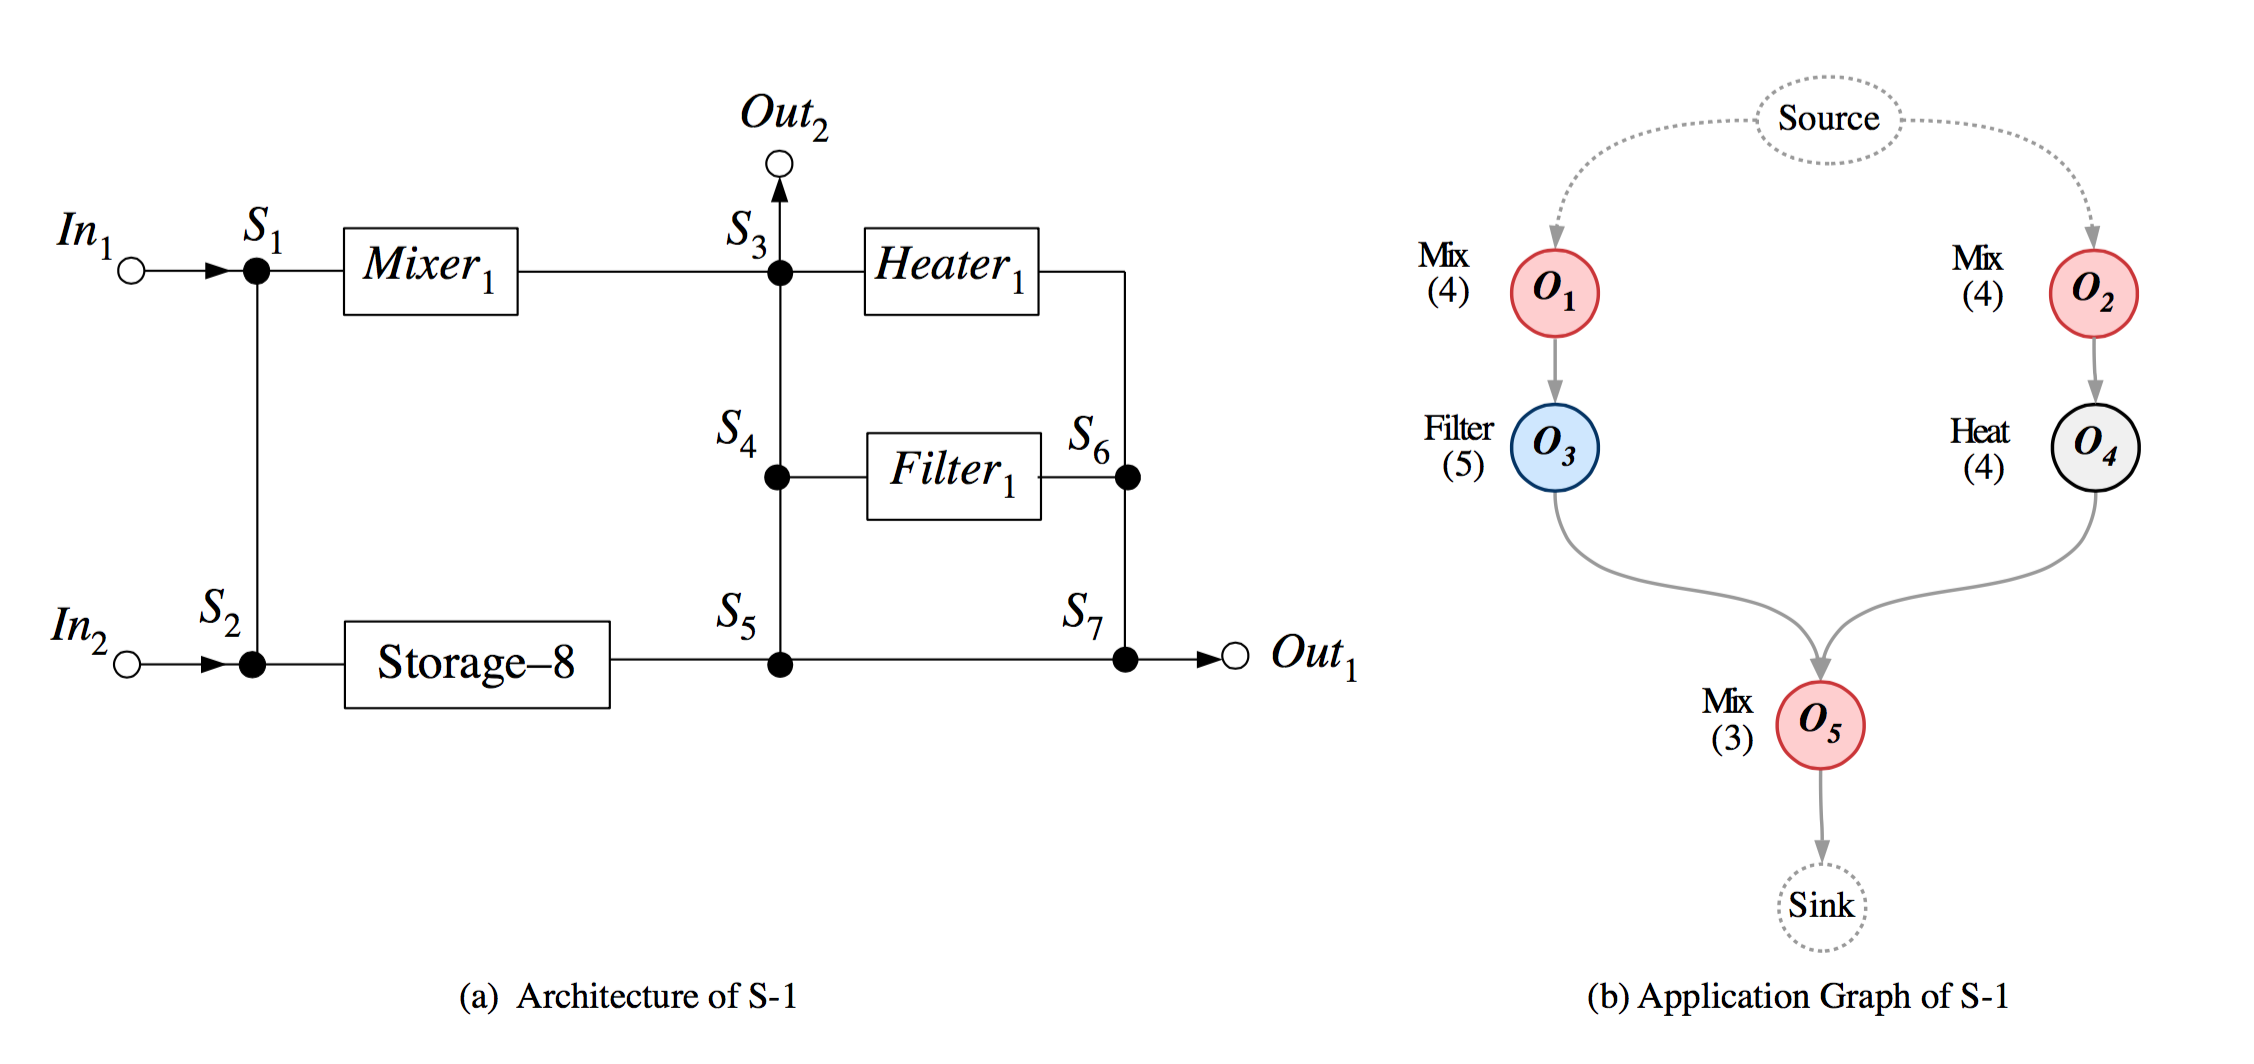
\includegraphics[scale=0.3]{figures/benchmark-s-1.png}
\caption[Architecture and application graph of S-1]{Architecture and application graph of S-1}
\label{fig:app-arch-s-1}
\end{figure}

S-1 is a synthetic benchmark. The architecture for S-1 is shown in \autoref{fig:app-arch-s-1}a and application graph for S-1 is shown in \autoref{fig:app-arch-s-1}b (5 operations).\\
The fault model for S-1 is: $\mathcal{Z} = (\mathcal{VF}, \mathcal{CF}, 2, 2)$ where $\mathcal{VF}$ and $\mathcal{CF}$ are shown in \autoref{tab:s-1-vf} and \autoref{tab:s-1-cf}, respectively.

\begin{table}[H]
\centering
\caption{The set of valve faults $\mathcal{VF}$ for S-1}
\begin{tabular}{| c | c | c | c |}
\hline
\textbf{Name} & \textbf{Vertex} ($N \in \mathcal{N})$ & \textbf{Valve affected} $(w)$ & \textbf{Type} $(t)$ \\ \hline
$VF_1$ & $Mixer_1$ & $v_5$ & Open \\ \hline
$VF_2$ & $S_6$ & $v_3$ & Open \\ \hline
$VF_3$ & $S_5$ & $v_2$ & Open \\ \hline
$VF_4$ & $S_3$ & $v_3$ & Open \\ \hline
\end{tabular}
\label{tab:s-1-vf}
\end{table}

\begin{table}[H]
\centering
\caption{The set of channel faults $\mathcal{CF}$ for S-1}
\begin{tabular}{| c | c | c | c |}
\hline
\textbf{Name} & \textbf{Component} ($M \in \mathcal{N}, \notin \mathcal{S})$ \textbf{/ Connection} $D_{i, j} \in \mathcal{D}$ & \textbf{Type} $(t)$ \\ \hline
$CF_1$ & $Heater_1$ & Block \\ \hline
$CF_2$ & $Filter_1$ & Block \\ \hline
$CF_3$ & $S_2 \rightarrow$ Storage-8 & Block \\ \hline
$CF_4$ & $S_1 \rightarrow Mixer_1$ & Block \\ \hline
\end{tabular}
\label{tab:s-1-cf}
\end{table}

\subsection{PCR Benchmark}
\begin{figure}[H]
\centering
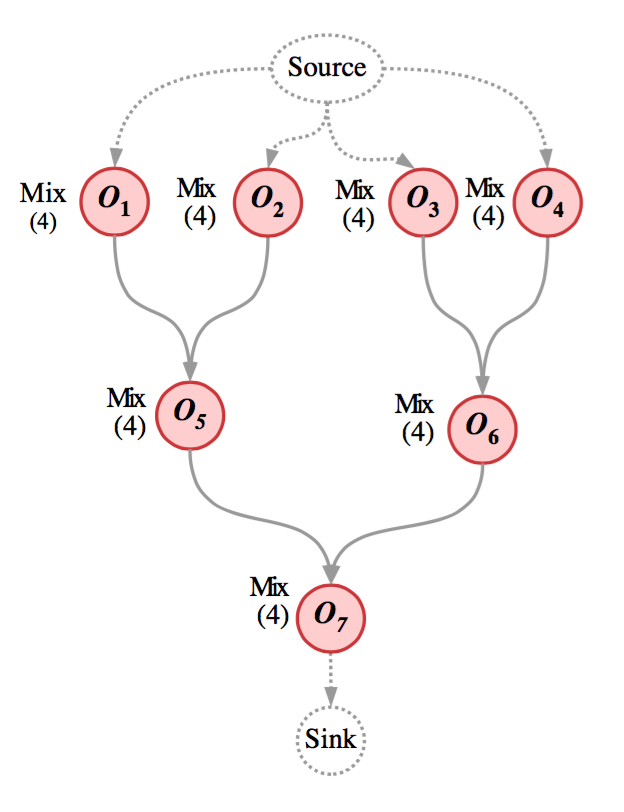
\includegraphics[scale=0.3]{figures/pcr-application.png}
\caption[Application graph for PCR]{Application graph of PCR}
\label{fig:pcr-app}
\end{figure}

Polymerase Chain Reaction, henceforth \emph{PCR}, is a real-life benchmark. The application graph for PCR is shown in \autoref{fig:pcr-app} (7 operations). The PCR architecture consists of 2 input nodes, 2 output nodes, 2 mixers, 1 storage component and 7 switches.\\
The fault model for PCR is: $\mathcal{Z} = (\mathcal{VF}, \mathcal{CF}, 2, 2)$ where $\mathcal{VF}$ and $\mathcal{CF}$ are shown in \autoref{tab:pcr-vf} and \autoref{tab:pcr-cf}, respectively.

\begin{table}[H]
\centering
\caption{The set of valve faults $\mathcal{VF}$ for PCR}
\begin{tabular}{| c | c | c | c |}
\hline
\textbf{Name} & \textbf{Vertex} ($N \in \mathcal{N})$ & \textbf{Valve affected} $(w)$ & \textbf{Type} $(t)$ \\ \hline
$VF_1$ & $Mixer_1$ & $v_5$ (pump) & Open \\ \hline
$VF_2$ & $Mixer_2$ & $v_6$ (pump) & Open \\ \hline
$VF_3$ & $S_1$ & $v_2$ (towards $S_2$) & Open \\ \hline
$VF_4$ & $S_3$ & $v_3$ (towards Storage1) & Open \\ \hline
\end{tabular}
\label{tab:pcr-vf}
\end{table}

\begin{table}[H]
\centering
\caption{The set of channel faults $\mathcal{CF}$ for PCR}
\begin{tabular}{| c | c | c | c |}
\hline
\textbf{Name} & \textbf{Component} ($M \in \mathcal{N}, \notin \mathcal{S})$ \textbf{/ Connection} $D_{i, j} \in \mathcal{D}$ & \textbf{Type} $(t)$ \\ \hline
$CF_1$ & $S_4 \rightarrow S_7$ & Block \\ \hline
$CF_2$ & $Mixer_1 \rightarrow S_3$ & Block \\ \hline
$CF_3$ & $S_5 \rightarrow Mixer_1$ & Block \\ \hline
\end{tabular}
\label{tab:pcr-cf}
\end{table}

\subsection{IVD Benchmark}
\begin{figure}[H]
\centering
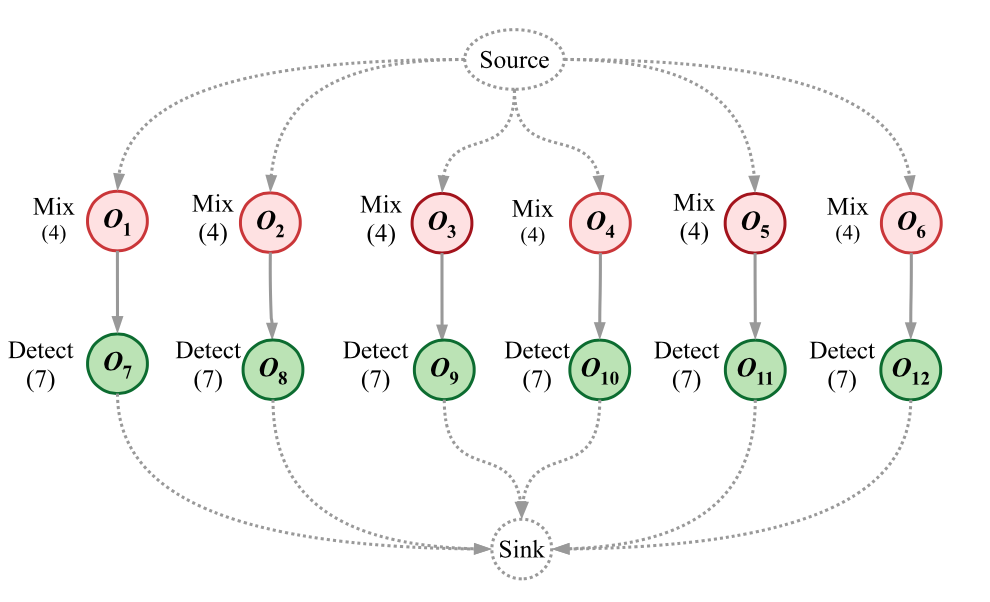
\includegraphics[scale=0.4]{figures/ivd-application.png}
\caption[Application graph of IVD \cite{wajid}]{Application graph of IVD \cite{wajid}}
\label{fig:ivd-app}
\end{figure}

In-vitro Diagnostics, henceforth \emph{IVD}, is a real-life benchmark. The application graph for IVD is shown in \autoref{fig:ivd-app} (12 operations). The IVD architecture consists of 2 input nodes, 2 output nodes, 2 mixers, 2 detectors, 1 storage component and 43 switches.\\
The fault model for PCR is: $\mathcal{Z} = (\mathcal{VF}, \mathcal{CF}, 2, 2)$ where $\mathcal{VF}$ and $\mathcal{CF}$ are shown in \autoref{tab:ivd-vf} and \autoref{tab:ivd-cf}, respectively.

\begin{table}[H]
\centering
\caption{The set of valve faults $\mathcal{VF}$ for IVD}
\begin{tabular}{| c | c | c | c |}
\hline
\textbf{Name} & \textbf{Vertex} ($N \in \mathcal{N})$ & \textbf{Valve affected} $(w)$ & \textbf{Type} $(t)$ \\ \hline
$VF_1$ & $Mixer_2$ & $v_5$ (pump) & Open \\ \hline
$VF_2$ & $S_{23}$ & $v_3$ (towards $S_{14}$) & Open \\ \hline
$VF_3$ & $S_{42}$ & $v_2$ (towards $Detector_2$) & Open \\ \hline
$VF_4$ & $S_2$ & $v_3$ (towards Storage1) & Open \\ \hline
$VF_5$ & $S_5$ & $v_3$ (towards $S_{15}$) & Open \\ \hline
$VF_6$ & $S_{10}$ & $v_2$ (towards $S_3$) & Open \\ \hline
$VF_7$ & $S_3$ & $v_1$ (towards $S_{21}$) & Open \\ \hline
\end{tabular}
\label{tab:ivd-vf}
\end{table}

\begin{table}[H]
\centering
\caption{The set of channel faults $\mathcal{CF}$ for IVD}
\begin{tabular}{| c | c | c | c |}
\hline
\textbf{Name} & \textbf{Component} ($M \in \mathcal{N}, \notin \mathcal{S})$ \textbf{/ Connection} $D_{i, j} \in \mathcal{D}$ & \textbf{Type} $(t)$ \\ \hline
$CF_1$ & $Detector_1$ & Block \\ \hline
$CF_2$ & $Detector_2$ & Block \\ \hline
$CF_3$ & $S_9 \rightarrow Detector_2$ & Block \\ \hline
$CF_4$ & $Mixer_1$ & Block \\ \hline
$CF_5$ & $S_{21} \rightarrow S_{28}$ & Block \\ \hline
$CF_6$ & $S_{16} \rightarrow S_5$ & Block \\ \hline
$CF_7$ & Storage1 & Block \\ \hline
\end{tabular}
\label{tab:ivd-cf}
\end{table}

\section{Solution Quality}
The parameters of which to evaluate fault-tolerant architectures depend on many factors. Two of the important factors are that we have to be able to reach every component on the chip (connectivity) and that the application has to be able to complete on the chip, even in the presence of any fault scenario possible under the given fault model. Meanwhile the physical constraints of the biochip also have to be considered as the physical size of the biochip should be kept as small as possible. Otherwise it would be easy to introduce fault-tolerance as we could just introduce many redundant components. Therefore the fault-tolerant architecture produced should be evaluated according to these three parameters, and the parameters are also considered by the objective function outlined in \autoref{chap:arch-eval}. A more practical and equally important feature considering solution quality is the yield of the biochips, i.e. the number of fabricated biochips that, after testing, are considered fault-tolerant hence they can be used by the end-users. Note that in principle, when introducing fault-tolerance to a given fault model, all the manufactured biochips should be fault-tolerant, so the yield should be 100\%. However, in practice, it may happen that after testing we detect a fault which is not captured by the fault model. Also, since our solution is based on a metaheuristic that uses a subset of the possible fault scenarios to decide on introducing redundancy, it may happen that the fault-tolerant biochip design is actually not tolerant to all the possible fault scenarios from the fault model.

The experiments evaluating solution quality are divided into two sets of experiments. The first set of experiments have the purpose to evaluate the quality of the obtained solutions and compare SA and GRASP. The second set of experiments will evaluate the yield of the obtained solutions.

\subsection{Objective Function Evaluation}
The initial features of the benchmarks are presented in \autoref{tab:1st-initial}. In \autoref{tab:1st-initial} $|\mathcal{N}|$ is the number of components, $|\mathcal{D}|$ is the number of connections, the cost is the number of valves and connections, the objective function calculated cost, Obj$_{cost}$ of the initial architecture $\mathcal{A}_{initial}$, the number of possible fault scenarios, the number of fault scenarios, $|\mathcal{FS}|$, generated for the specific benchmark, and $d_{\mathcal{G}}$ denotes the deadline for the application. Note that the Obj$_{cost}$ of the initial architecture is quite high due to the penalty values of the objective function.

\begin{table}[H]
\centering
\caption{The benchmarks and their initial features}
\begin{tabular}{| c | c | c  c  c c | c | c | c |}
\hline
\multirow{2}{*}{Name} &
\multirow{2}{*}{Type} &
\multicolumn{4}{ c |}{$\mathcal{A}_{initial}$} &
\multirow{2}{*}{Possible $|\mathcal{FS}|$} &
\multirow{2}{*}{$|\mathcal{FS}|$} &
\multirow{2}{*}{$d_\mathcal{G}$} \\
%\multicolumn{4}{c}{$\mathcal{A}_{SA}$} &
%\multicolumn{4}{c}{$\mathcal{A}_{GRASP}$} \\ 
& & {$|\mathcal{N}|$} & {$|\mathcal{D}|$} & Cost & {Obj$_{cost}$} & & &  \\ \hline %& {Components} & {FT-components} & {Connections} & {Cost} & {Components} & {FT-components} & {Connections} & {Cost} \\ \hline
S-1 & Synthetic & 15 & 17 & 84 & 22350084 & 121 & 100 & 50  \\ \hline
PCR & Real-life & 14 & 16 & 88 & 1695088 & 77 & 50 & 65  \\ \hline
IVD & Real-life & 52 & 78 & 274 & 1800274 & 841 & 100 & 90  \\ \hline
%Name & Type & $\mathcal{A}_{initial}$ & Number of components &  \\ \hline
\end{tabular}
\label{tab:1st-initial}
\end{table}

In \autoref{tab:1st-result} the resulting fault-tolerant netlists are presented. The specifications are the same as in \autoref{tab:1st-initial} with the addition that FT-$|\mathcal{N}|$ is the number of fault-tolerant components. The netlist obtained by Simulated Annealing is denoted as $\mathcal{A}_{SA}$ and the netlist obtained by GRASP is denoted as $\mathcal{A}_{GRASP}$. The initial netlists and the resulting netlists are shown in \autoref{app:netlists} where they are drawn using GraphViz.

\begin{table}[H]
\centering
\caption{The resulting fault-tolerant netlist of the benchmarks}
\begin{tabular}{| c | c  c  c  c | c  c  c c | c c c c c c}
\hline
\multirow{2}{*}{Name} &
\multicolumn{4}{c |}{$\mathcal{A}_{SA}$} &
\multicolumn{4}{c |}{$\mathcal{A}_{GRASP}$} \\
& {$|\mathcal{N}|$}  & {FT-$|\mathcal{N}|$} & {$|\mathcal{D}|$} & {Cost}
& {$|\mathcal{N}|$}  & {FT-$|\mathcal{N}|$} & {$|\mathcal{D}|$} & {Cost} 
\\ \hline
S-1 & 24 & 1 & 35 & 185 & 15 & 3 & 20 & 102 \\ \hline
PCR & 19 & 1 & 27 & 124 & 14 & 1 & 17 & 92 \\ \hline
IVD & 53 & 2 & 80 & 285 & 52 & 2 & 78 & 279 \\ \hline

\end{tabular}
\label{tab:1st-result}
\end{table}

These experiments show that both algorithms have been able to find a solution deemed fault-tolerant by using the same cost function presented in \autoref{chap:arch-eval}. This is the case for all benchmarks used. Thereby a fault-tolerant architecture has been synthesised for each benchmark such that the architecture is connected and the application can complete within its deadline considering their respective fault models.

In terms of obtaining a less costly fault-tolerant netlist GRASP performs better than SA in all benchmarks. However considering the IVD benchmark the algorithms perform almost equally. GRASP uses less components and connections to obtain a fault-tolerant solution and thereby the cost of the solutions are smaller for GRASP. On average the cost of the solutions found by GRASP are 20\% less costly than the solutions found by SA. A possible reason that SA does worse than GRASP is that SA performs a number of bad moves in order to converge towards the global optimum, where the moves are hard to recover from. However, this requires further investigation in order to determine the exact reasons.

%The reason behind GRASP finding better solutions needs further investigation. Although one possibility is that SA performs a number of bad moves in order to converge towards the global optimum, where the moves are hard to recover from.

\subsection{Yield Evaluation}
\label{sec:yield-eval}
In this set of experiments only one benchmark is used, which is S-1. Furthermore it will use only one algorithm to evaluate the yield. The algorithm used is GRASP considering it performed better than SA in the first set of experiments. The purpose of these experiments is evaluating the yield and the influence of the number of randomly generated fault scenarios on the obtained solution. The result of the experiments are given in \autoref{tab:yield-eval}. In \autoref{tab:yield-eval} $|\mathcal{N}|$ is the number of components, $|\mathcal{D}|$ is the number of connections, the objective function calculated cost is denoted by Obj$_{cost}$, the cost is the number of valves and connections, the initial architecture is denoted $\mathcal{A}_{initial}$, $\mathcal{A}_{result}$ is the resulting architecture, $|\mathcal{FS}|$ is the number of fault scenarios generated for the specific benchmark, $|FT|$ denotes the number of fault scenarios, $f \in \mathcal{FS}$, the resulting architecture tolerates, $|\neg FT|$ denotes the number of fault scenarios not tolerated and $FT\%$ is the percentage of fault scenarios tolerated.

\begin{table}[H]
\centering
\caption{The benchmark and the yield evaluation thereof}
\begin{tabular}{| c c c | c | c c  c  c | c | c | c | c | c | c |}
\hline
%\multirow{2}{*}{Name} &
\multicolumn{3}{|  c |}{$\mathcal{A}_{initial}$} &
\multirow{2}{*}{$|\mathcal{FS}|$} &
\multicolumn{4}{c |}{$\mathcal{A}_{result}$} &
\multirow{2}{*}{$|FT|$} &
\multirow{2}{*}{$|\neg FT|$} &
\multirow{2}{*}{$FT\%$} \\
%\multicolumn{4}{c}{$\mathcal{A}_{GRASP}$} \\ 
% & 
{$|\mathcal{N}|$} & {$|\mathcal{D}|$} & {Obj$_{cost}$} & & {$|\mathcal{N}|$}  & {FT-$|\mathcal{N}|$} & {$|\mathcal{D}|$} & {Cost} & & & \\ \hline %& {Components} & {FT-components} & {Connections} & {Cost} & {Components} & {FT-components} & {Connections} & {Cost} \\ \hline
15 & 17 & 5760084 & 25 & 16 & 2 & 20 & 98 & 105 & 16  & 86.78 \\ \hline
15 & 17 & 10540084 & 50 & 15 & 3 & 19 & 99 & 117 & 4  & 96.69 \\ \hline
15 & 17 & 18580084 & 85 & 16 & 2 & 21 & 101 & 121 & 0 & 100 \\ \hline
15 & 17 & 27610084 & 121 & 15 & 3 & 19 & 99 & 121 & 0 & 100 \\ \hline
%Name & Type & $\mathcal{A}_{initial}$ & Number of components &  \\ \hline
\end{tabular}
\label{tab:yield-eval}
\end{table}

\autoref{tab:yield-eval} shows that the number of fault scenarios generated has some influence on the obtained solutions, although it is not a critical factor. When generating only 25 fault scenarios we obtain a solution that tolerates 86.78\% of the possible fault scenarios. This is because if a fault-tolerant solution in terms of the objective function, i.e. the application can be scheduled and the architecture is connected in all the generated fault scenarios, is found then it tolerates each individual fault in the fault scenarios. However the combination of certain faults will make the biochip unusable. This experiment shows that even generating a fraction of the possible fault scenarios can lead to good fault tolerance to all possible fault scenarios. In this case 21\% of the possible fault scenarios were generated and the percentage of fault scenarios tolerated is 86.78\%. By virtue of this it is possible to get good fault-tolerance results on large architectures where generating a large portion of the fault scenarios to use in the cost function would be computationally infeasible. Furthermore the experiment also shows that it is able to obtain a fault-tolerance of 100\% to the possible fault scenarios when generating 70\% percent of the fault scenarios. Thus the yield can be increased considerably by using the tool in developed in this thesis.

%Thus in order to increase the yield the number of fault scenarios generated should be such that a good portion of the possible fault scenarios are generated. In this experiment a yield of 100\% was found by generating 70\% (85) of the possible fault scenarios. Thus generating 70-75\% of the possible fault scenarios should be sufficient to obtain a yield of 100\% considering the fault model given as input.


\section{Performance}
In \autoref{tab:performance-exp} the running time of the experiments presented earlier are outlined. The number of vertices in initial architecture $\mathcal{A}_{initial}$ are denoted as $|\mathcal{N}|$ and the number of connections is $|\mathcal{D}|$. The number of operations in the application graph $\mathcal{G}$ are denoted as $|\mathcal{O}|$ and the number of generated fault scenarios for the benchmarks are denoted as $|\mathcal{FS}|$. $\mathcal{A}_{SA}$ describes the running time of Simulated Annealing where the time is presented as hh:mm:ss. $\mathcal{A}_{GRASP}$ presents the running time of GRASP with the same time formatting as $\mathcal{A}_{SA}$. Note that test 2, 3, 4 and 5 in the table has no running time for SA as these benchmarks were only evaluated with GRASP in \autoref{sec:yield-eval}.

\begin{table}[H]
\centering
\caption{The benchmarks and their performance}
\begin{tabular}{| c | c | c | c  c | c | c | c | c |}
\hline
\multirow{2}{*}{\#} &
\multirow{2}{*}{Name} &
\multirow{2}{*}{Type} &
\multicolumn{2}{ c |}{$\mathcal{A}_{initial}$} &
\multirow{2}{*}{$|\mathcal{O}|$} &
\multirow{2}{*}{$|\mathcal{FS}|$} &
\multirow{2}{*}{$\mathcal{A}_{SA}$} &
\multirow{2}{*}{$\mathcal{A}_{GRASP}$} \\
& & & {$|\mathcal{N}|$} & {$|\mathcal{D}|$} & & & &  \\ \hline %& {Components} & {FT-components} & {Connections} & {Cost} & {Components} & {FT-components} & {Connections} & {Cost} \\ \hline
1 & S-1 & Synthetic & 15 & 17 & 5 & 100 & 06:23:54 & 01:22:36  \\ \hline
2 & S-1 & Synthetic & 15 & 17 & 5 & 25 & - & 00:23:23  \\ \hline
3 & S-1 & Synthetic & 15 & 17 & 5 & 50 & - & 00:45:23  \\ \hline
4 & S-1 & Synthetic & 15 & 17 & 5 & 85 & - & 01:15:45  \\ \hline
5 & S-1 & Synthetic & 15 & 17 & 5 & 121 & - & 01:43:26  \\ \hline
6 & PCR & Real-life & 14 & 16 & 7 & 50 & 16:05:57 & 02:23:52  \\ \hline
7 & IVD & Real-life & 52 & 78 & 12 & 100  & 184:50:28 & 27:40:37 \\ \hline
%Name & Type & $\mathcal{A}_{initial}$ & Number of components &  \\ \hline
\end{tabular}
\label{tab:performance-exp}
\end{table}

\autoref{tab:performance-exp} shows that the running time of GRASP is much faster than SA in all benchmarks. Part of the reason is that SA uses the objective function at each iteration whereas GRASP uses it only in the local search and furthermore SA with a slow temperature cooling schedule will have more iterations than the main loop of GRASP. The objective function is the computationally slow part of the algorithms. However GRASP still does considerably better in terms of running time. Considering the S-1 benchmark GRASP is approximately 4 times faster than SA. GRASP finds a solution to the PCR benchmark approximately 6-7 times faster than SA. Similarly with the IVD benchmark where GRASP finds a solution 7-8 times faster than SA. Therefore it can be concluded that GRASP does substantially better performance-wise in the benchmarks. However there could be implemented optimisations of the objective function that would benefit the running time of both algorithms.

\section{Summary}
In this chapter the algorithms proposed for the fault-tolerant architecture synthesis problem have been evaluated by applying them to three different benchmarks. The evaluation was done in terms of solution quality and performance, where GRASP did considerably better than SA in both categories. Furthermore in an effort to increase the yield even generating a fraction of the possible fault scenarios provides good fault-tolerance on all possible fault scenarios.